

%\newcommand{\ANIMATEGRAPHICS}[5]{\animategraphics[#1]{#2}{#3}{#4}{#5}}
\newcommand{\ANIMATEGRAPHICS}[5]{ANIMATION: #3}

%========================================================================
% UNCOMMENT TO PRINT
%========================================================================

 \newcommand{\PAUSE}{}
 \newcommand{\enhance}[1]{}
 \newcommand{\enhancebf}[2]{\textbf{#2}}
 \newcommand{\enhanceus}[1]{\color{blue}}
 \newcommand{\enhancenewus}[1]{\color{magenta}}
 \newcommand{\enhancethem}[1]{\color{red!50!black}}
 \newcommand{\ENHANCE}[1]{
  \temporal<#1>{\color{lightgray}}{\color{black}}{\color{gray}}}

%========================================================================
% UNCOMMENT FOR PRESENTATION:
%========================================================================

% \newcommand{\PAUSE}{\pause}
% \newcommand{\enhance}[1]{\temporal<#1>{\color{lightgray}}{\color{black}}{\color{black}}}
% \newcommand{\enhancebf}[2]{\enhance{#1}\textbf{#2}}
% \newcommand{\enhanceus}[1]{\temporal<#1>{\color{lightgray}}{\color{blue}}{\color{blue}}}
% \newcommand{\enhancenewus}[1]{\temporal<#1>{\color{lightgray}}{\color{magenta}}{\color{magenta}}}
%\newcommand{\enhancethem}[1]{\temporal<#1>{\color{lightgray}}{\color{red!50!black}}{\color{red!50!black}}}
% \newcommand{\ENHANCE}[1]{
% \temporal<#1>{\color{lightgray}}{\color{black}}{\color{black}}}
%========================================================================

% UNCOMMENT FOR HANDOUT 
\documentclass[xcolor=table,slidestop,compress,handout]{beamer}
% UNCOMMENT FOR PRESENTATION
%\documentclass[xcolor=table,slidestop,compress]{beamer}

%\documentclass[xcolor=table,compress]{beamer}

\DeclareFontShape{OT1}{cmtt}{bx}{n}{<5><6><7><8><9><10><10.95><12><14.4><17.28><20.74><24.88>cmttb10}{}
\usepackage{mathtools}

\DeclarePairedDelimiter\abs{\lvert}{\rvert}%
\DeclarePairedDelimiter\norm{\lVert}{\rVert}%

%----------------------------------------------------------------------
% For TIKZ flow chart diagrams
\usepackage[latin1]{inputenc}
\usepackage{tikz}
\usetikzlibrary{shapes,arrows}
%----------------------------------------------------------------------

\usepackage[T1]{fontenc}
\usepackage{listings}
\usepackage{bm}
\usepackage{alltt}
\usepackage[overlay]{textpos}
%\usepackage{MnSymbol,wasysym}  % MnSymbol breaks |x|
\usepackage{wasysym}
\usepackage{animate}
\usepackage{minted}
\usepackage[small]{eulervm}
\usepackage{fancybox}
\usepackage{hyperref}

%\usepackage{sphinx}


%\usetheme{Copenhagen}
\usetheme{Luebeck}
%\usetheme{Szeged}
%\usetheme{Montpellier}
%\usetheme{Madrid}
%\usetheme{Warsaw}
%\usetheme{CambridgeUS}

%\useinnertheme{default}
\useoutertheme{infolines}

\newcommand{\icon}{\large{$\bigtriangleup$}}
%\logo{\hfill\hyperlink{titlepage<1>}{\icon}}
%\usecolortheme{default}
%\usecolortheme{sidebartab}
\setbeamersize{text margin left = 0.25in}
%\setbeamercolor{structure}{fg=cyan!90!black}
\usecolortheme{spruce} 
%\usecolortheme{lily} 
%\usecolortheme{dove} % black and white

\newcommand{\etc}{\vspace{-0.05in}\centerline{\dots}\vspace{-0.10in}}
\newcommand{\todo}{$\bigcirc$}

\newcommand{\BUTTON}[1]{#1}
\newcommand{\link}[2]{\hyperlink{#1}{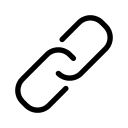
\includegraphics[height=0.1in]{icon-link.png}\underline{\greentext{#2}}}}


%\newcommand{\sINTRO}{Enzo-P / Cello Project Summary}

%==================================================
\newcommand{\ssPurpose}{What is the purpose of this document?}

%==================================================
\newcommand{\sIntro}{What is Enzo-P/Cello?}
\newcommand{\ssMotivation}{Why does Enzo-P exist?}
\newcommand{\ssAmr}{How does Enzo-P's AMR differ from Enzo's?}
\newcommand{\ssCompare}{How do Enzo-P and Enzo differ?}
\newcommand{\ssApproach}{How does Enzo-P address Enzo's limitations?}

\newcommand{\sRecent}{New features}
\newcommand{\ssRecentCosmology}{Cosmology}
\newcommand{\ssRecentParticles}{Abstract particles}
\newcommand{\ssRecentGravity}{Scalable gravity}
\newcommand{\ssRecentHistory}{Old fields}
\newcommand{\ssRecentTemporary}{Temporary fields}

\newcommand{\sSoon}{Coming soon\ldots}
\newcommand{\ssSoonIo}{MUSIC I.C.'s}
\newcommand{\ssSoonYt}{yt support}
\newcommand{\ssSoonUnits}{Units}

%==================================================
\newcommand{\sCharm}{\charm\ system}
\newcommand{\ssCharm}{What is \charm?}
\newcommand{\ssCharmCode}{How do I write a simple \charm\ program?}
\newcommand{\ssCharmPup}{\charm\ ``pup'' functions--what are they?}
\newcommand{\ssCharmCello}{How is \charm\ used in Cello?}
%==================================================
\newcommand{\sDesign}{Software design}

\newcommand{\ssOop}{Design overview}
\newcommand{\ssComponents}{Cello software components}
\newcommand{\ssClasses}{Enzo-P / Cello classes}
\newcommand{\ssSimulation}{Simulation classes}
\newcommand{\ssProblems}{Problem classes}
\newcommand{\ssBlocks}{Block and Data classes}
%\newcommand{\ssData}{The Data class}
\newcommand{\ssFields}{Field data classes}
\newcommand{\ssParticles}{Particle data classes}
\newcommand{\ssMethods}{Method classes}
\newcommand{\ssInitialBoundary}{Initial and Boundary conditions classes}
\newcommand{\ssRefine}{Mesh refinement criteria classes}
%\newcommand{\ssStopping}{Stopping criteria class}
%\newcommand{\ssClassesOrg}{How are Enzo-P's classes organized?}

%==================================================
\newcommand{\sDevel}{Developing Enzo-P}

%\newcommand{\sCODE}{Enzo-P / Cello Source Code Design and Implementation}
\newcommand{\ssDevelCoding}{Enzo-P develper coding guidelines and suggestions}
\newcommand{\ssDevelParameter}{How do I add a new input parameter?}
\newcommand{\ssDevelMethod}{How do I add a new method?}
\newcommand{\ssDevelFields}{How do I write a Method using Fields?}
\newcommand{\ssDevelParticles}{How do I write a Method using Particles?}
\newcommand{\ssDevelInitial}{How do I add initial conditions?}
\newcommand{\ssDevelBoundary}{How do I add new boundary conditions?}
\newcommand{\ssDevelRefine}{How do I add a new refinement criterium?}
\newcommand{\ssDevelTest}{How do I add a new unit test program?}

%==================================================
\newcommand{\sFuture}{Future directions}

\newcommand{\ssRoadmap}{What is the project roadmap?}
\newcommand{\ssFutureHydro}{Unfinished business: hydrodynamics}
\newcommand{\ssFutureGravity}{Unfinished business: gravity}
\newcommand{\ssFutureChemistry}{Unfinished business: chemistry}
\newcommand{\ssFutureParticles}{Unfinished business: particles}
\newcommand{\ssFutureMagnetism}{Unfinished business:  MHD}
\newcommand{\ssFutureRadiation}{Unfinished business: radiation}
\newcommand{\ssContribute}{How can I contribute?}

%==================================================
\newcommand{\sParameters}{Parameter files}

\newcommand{\ssParamIntro}{Enzo-P/Cello parameter files}
\newcommand{\ssParameters}{Writing Enzo-P parameter files}
\newcommand{\ssDoubleMach}{Case Study: Double Mach Reflection}
\newcommand{\ssParamActivity}{Getting to know Enzo-P better}

\newcommand{\ssCharmSummary}{Summary}
\newcommand{\ssControlSummary}{Summary}
\newcommand{\ssDesignSummary}{Summary}
\newcommand{\ssDevelSummary}{Summary}
\newcommand{\ssFutureSummary}{Summary}
\newcommand{\ssIntroSummary}{Summary}
\newcommand{\ssParametersSummary}{Summary}
\newcommand{\ssPresentSummary}{Summary}
\newcommand{\ssRecentSummary}{Summary}
\newcommand{\ssProjectSummary}{Summary}
\newcommand{\ssStartingSummary}{Summary}

%\newcommand{\ssParamProblem}{What parameters are available for defining problems?}
%\newcommand{\ssParamRefine}{What parameters are available for controling mesh refinement?}
%\newcommand{\ssParamData}{What parameters are available for defining data structures?}
%\newcommand{\ssParamMethod}{What parameters are available for specifying numerical methods?}
%\newcommand{\ssParamIo}{What parameters are available for controling I/O?}
%\newcommand{\ssParamOther}{What other parameters are available?}

%==================================================
\newcommand{\sControl}{Control flow}

\newcommand{\ssControl}{How are phases of the computation controlled?}
\newcommand{\ssAdapt}{Adaptive Mesh Refinement}
\newcommand{\ssRefresh}{Refresh ghost zones}

%==================================================
\newcommand{\sPresent}{Current status}

\newcommand{\ssState}{What is the current status of Enzo-P/Cello?}
\newcommand{\ssCurrent}{What are Enzo-P's current capabilities?}
\newcommand{\ssScaling}{How well does Enzo-P scale?}
\newcommand{\ssIssues}{What are some of Enzo-P's known issues?}

%==================================================
\newcommand{\sProject}{Project organization}

\newcommand{\ssProject}{How is the Enzo-P project currently organized?}
\newcommand{\ssSource}{Where is the source code hosted?}
\newcommand{\ssBrowse}{How can I browse the source code?}
\newcommand{\ssDocumentation}{What documentation is available?}
\newcommand{\ssBugs}{What are some of the known bugs?}
\newcommand{\ssTesting}{How is testing done?}
%\newcommand{\ssCommunicate}{How do Enzo-P developers communicate?}

%==================================================
\newcommand{\sStarting}{Getting started}

\newcommand{\ssStarting}{Getting started using Enzo-P / Cello}
\newcommand{\ssInstallCharm}{How do I download and install Charm++?}
\newcommand{\ssInstallEnzop}{How do I download Enzo-P?}
\newcommand{\ssConfigure}{How do I configure Enzo-P?}
\newcommand{\ssCompile}{How do I compile Enzo-P?}
\newcommand{\ssRunning}{How do I run an example problem?}
%\newcommand{\ssDoubleMach}{Double Mach Reflection}
\newcommand{\ssRestart}{How do I restart from a checkpoint?}
\newcommand{\ssLoadBalance}{How do I run with dynamic load balancing?}
\newcommand{\ssTools}{What tools does Cello provide?}


%==================================================
\newcommand{\sTemplate}{TEMPLATE SECTION TITLE}
%==================================================

\newcommand{\orow}[1]{\textcolor{blue}{#1}}
\newcommand{\erow}[1]{\textcolor{blue!50!black}{#1}}

\newcommand{\blockred}{\setbeamercolor{block title}{bg=red!30,fg=black}}
\newcommand{\blockgreen}{\setbeamercolor{block title}{bg=green!30,fg=black}}
\newcommand{\blockblue}{\setbeamercolor{block title}{bg=blue!30,fg=black}}

\newcommand{\bad}{\textcolor{red}{\frownie}}
\newcommand{\good}{\textcolor{green}{\smiley}}
\newcommand{\blck}{\code{Block}}
\newcommand{\cello}{\textsf{Cello}}
\newcommand{\charm}{{\sf Charm\pp}}

\newcommand{\code}[1]{\texttt{#1}}


\newcommand{\yellowcode}[1]{\textcolor{yellow!50!black}{\code{#1}}}
\newcommand{\greycode}[1]{\textcolor{grey}{\code{#1}}}
\newcommand{\cyancode}[1]{\textcolor{cyan!50!black}{\code{#1}}}

\newcommand{\urltext}[1]{\greentext{\url{#1}}}
\newcommand{\bluecode}[1]{\textcolor{blue}{\code{#1}}}
\newcommand{\greencode}[1]{\textcolor{green!50!black}{\code{#1}}}
\newcommand{\redcode}[1]{\textcolor{red!50!black}{\code{#1}}}
\newcommand{\magentacode}[1]{\textcolor{magenta}{\code{#1}}}
\newcommand{\purplecode}[1]{\textcolor{purple!70!black}{\code{#1}}}
\newcommand{\orangecode}[1]{\textcolor{orange!60!black}{\code{#1}}}

\newcommand{\greyit}[1]{\textcolor{grey}{\textit{#1}}}
\newcommand{\cyanit}[1]{\textcolor{cyan!50!black}{\textit{#1}}}
\newcommand{\blueit}[1]{\textcolor{blue}{\textit{#1}}}
\newcommand{\greenit}[1]{\textcolor{green!50!black}{\textit{#1}}}
\newcommand{\redit}[1]{\textcolor{red!50!black}{\textit{#1}}}
\newcommand{\magentait}[1]{\textcolor{magenta!70!black}{\textit{#1}}}
\newcommand{\orangeit}[1]{\textcolor{orange!60!black}{\textit{#1}}}

\newcommand{\redtext}[1]{\textcolor{red!70!black}{#1}}
\newcommand{\cyantext}[1]{\textcolor{cyan!50!black}{#1}}
\newcommand{\orangetext}[1]{\textcolor{orange!60!black}{#1}}
\newcommand{\yellowtext}[1]{\textcolor{yellow!50!black}{#1}}
\newcommand{\greentext}[1]{\textcolor{green!50!black}{#1}}
\newcommand{\bluetext}[1]{\textcolor{blue}{#1}}
\newcommand{\magentatext}[1]{\textcolor{magenta!70!black}{#1}}

\newcommand{\addclass}[1]{\bluetext{#1}}
\newcommand{\addconstruct}[1]{\cyantext{#1}}
\newcommand{\addparam}[1]{\magentatext{#1}}
\newcommand{\addcharm}[1]{\redtext{#1}}
\newcommand{\addtest}[1]{\greentext{#1}}

\newcommand{\addclassbf}[1]{\bluetext{\textbf{#1}}}
\newcommand{\addconstructbf}[1]{\cyantext{\textbf{#1}}}
\newcommand{\addparambf}[1]{\magentatext{\textbf{#1}}}
\newcommand{\addcharmbf}[1]{\redtext{\textbf{#1}}}
\newcommand{\addtestbf}[1]{\greentext{\textbf{#1}}}

\newcommand{\redcirc}{\textcolor{red!50!black}{$\bigcirc$}}
\newcommand{\orangecirc}{\textcolor{orange!60!black}{$\bigcirc$}}
\newcommand{\yellowcirc}{\textcolor{yellow!50!black}{$\bigcirc$}}
\newcommand{\greencirc}{\textcolor{green!50!black}{$\bigcirc$}}
\newcommand{\bluecirc}{\textcolor{blue}{$\bigcirc$}}
\newcommand{\magentacirc}{\textcolor{magenta!70!black}{$\bigcirc$}}


\newcommand{\redbf}[1]{\textcolor{red!50!black}{\textbf{#1}}}
\newcommand{\cyanbf}[1]{\textcolor{cyan!50!black}{\textbf{#1}}}
\newcommand{\orangebf}[1]{\textcolor{orange!60!black}{\textbf{#1}}}
\newcommand{\yellowbf}[1]{\textcolor{yellow!50!black}{\textbf{#1}}}
\newcommand{\greenbf}[1]{\textcolor{green!50!black}{\textbf{#1}}}
\newcommand{\bluebf}[1]{\textcolor{blue}{\textbf{#1}}}
\newcommand{\magentabf}[1]{\textcolor{magenta!70!black}{\textbf{#1}}}

\newcommand{\highpriority}{}
\newcommand{\medpriority}{}
\newcommand{\lowpriority}{}

\newcommand{\group}[1]{\bluecode{#1}}
\newcommand{\subgroup}[1]{\greencode{#1}}
\newcommand{\parameter}[1]{\redcode{#1}}
\newcommand{\valuetext}[1]{\cyancode{#1}}
\newcommand{\comment}[1]{\textsf{\textbf{\blueit{#1}}}}

\newcommand{\type}[1]{\greencode{#1}}
\newcommand{\variable}[1]{\orangecode{#1}}
\newcommand{\function}[1]{\bluecode{#1}}
\newcommand{\keyword}[1]{\purplecode{#1}}

\newcommand{\enzopcello}{\textsf{Enzo-P/Cello}}
\newcommand{\enzop}{\textsf{Enzo-P}}
\newcommand{\enzo}{\textsf{Enzo}}
\newcommand{\itemnum}[1]{\item<#1>}
\newcommand{\newus}[1]{\color{magenta!70!black}{#1}}
\newcommand{\patch}{\code{Patch}}
\newcommand{\pp}{\texttt{++}}
\newcommand{\seed}{\code{Seed}}
\newcommand{\seedgrid}{\code{SeedGrid}}
\newcommand{\seedtree}{\code{SeedTree}}
\newcommand{\them}[1]{\color{red!50!black}{#1}}
\newcommand{\tree}{\code{Tree}}
\newcommand{\us}[1]{\color{blue}{#1}}
\newcommand{\cursor}[1]{\uncover<#1>{\begin{animateinline}[autoplay,loop]{2.0}
\strut\textbf{\_}\newframe\newframe[5]
\end{animateinline}}}
\newcommand{\prompt}{\textcolor{blue!50!black}{\$}}
\newcommand{\bfat}[2]{\alt<#1>{\textbf{#2}}{#2}}
%\newcommand{\colorat}[2]{\textcolor<#1>{f{#2}}{#2}}
\newcommand{\TITLE}[2]{\title{#1}
\subtitle{#2}
\author[Bordner/Norman]{James Bordner \and Michael L.~Norman}
\institute {
   University of California, San Diego\\
   San Diego Supercomputer Center}
\date[2018-05-14/18]{Enzo Days 2018 / Georgia Tech \\
            2018-05-14/18}}

\definecolor{enzop}{rgb}{0.75,0.00,0.00}
\definecolor{cello}{rgb}{0.00,0.50,0.000}


% background color
% \beamersetaveragebackground{yellow!10}
\beamertemplatetransparentcoveredhigh
%\beamertemplatetransparentcovereddynamicmedium
%@@@@@@@@@@@@@@@@@@@@@@@@@@@@@@@@@@@@@@@@@@@@@@@@@@
% This removes paretheses around ``name (institution)'' in footer
%@@@@@@@@@@@@@@@@@@@@@@@@@@@@@@@@@@@@@@@@@@@@@@@@@@
\makeatletter
\setbeamertemplate{footline}
{
  \leavevmode%
  \hbox{%
  \begin{beamercolorbox}[wd=.333333\paperwidth,ht=2.25ex,dp=1ex,center]{author in head/foot}%
    \usebeamerfont{author in head/foot}\insertshortauthor%~~\beamer@ifempty{\insertshortinstitute}{}{(\insertshortinstitute)}
  \end{beamercolorbox}%
  \begin{beamercolorbox}[wd=.333333\paperwidth,ht=2.25ex,dp=1ex,center]{title in head/foot}%
    \usebeamerfont{title in head/foot}\insertshorttitle
  \end{beamercolorbox}%
  \begin{beamercolorbox}[wd=.333333\paperwidth,ht=2.25ex,dp=1ex,right]{date in head/foot}%
    \usebeamerfont{date in head/foot}\insertshortdate{}\hspace*{2em}
    \insertframenumber{} / \inserttotalframenumber\hspace*{2ex} 
  \end{beamercolorbox}}%
  \vskip0pt%
}
\makeatother

